\documentclass[tikz]{standalone}

\usepackage{amsfonts}
\usepackage{amsmath}
\usepackage{braket}

\usepackage{tikz}
\usetikzlibrary{shapes.geometric,patterns,positioning,matrix}
\usetikzlibrary{shadows,calc,3d,arrows.meta,decorations.pathmorphing,decorations.markings,decorations.pathreplacing}

\definecolor{googleB}{HTML}{4285F4}
\definecolor{googleG}{HTML}{34A853}
\definecolor{googleY}{HTML}{FBBC05}
\definecolor{googleR}{HTML}{EA4335}
\definecolor{googleBG}{HTML}{3B96A4}

% load TikZ grafic definitions
%\input{gfx_TikZ}

% main document
\begin{document}

	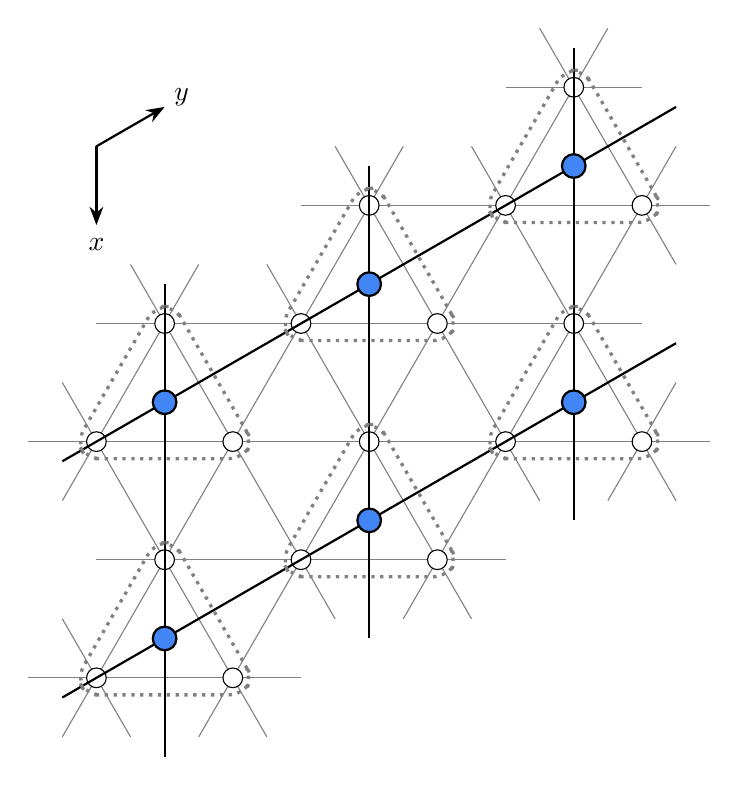
\begin{tikzpicture}

		\def\clipX{2.00}
		\def\clipY{1.75}
		\def\legLength{0.2}
		\def\tensorSize{0.125}
		\def\tensorSizeS{0.15}

		\begin{scope}[shift = {({3*cos(30)}, +5.25)}]
            \draw[thick, -{Stealth[scale = 1.0]}] (0 : 0) to (270 : 1.0) node at (270 : 1.25) {$x$};
            \draw[thick, -{Stealth[scale = 1.0]}] (0 : 0) to ( 30 : 1.0) node at ( 30 : 1.25) {$y$};
        \end{scope}

		% \begin{scope}[shift = {(-4.25,{0.5*cos(30)*tan(60)/2}) to (+2,{1*cos(30)*tan(60)/2})}]
		\begin{scope}[]

			\foreach \x/\y in {+3/-2, +6/0, +3/+2, +9/+2, +6/+4, +9/+6} {
				\begin{scope}[shift = {({\x*cos(30)}, {\y*cos(30)*tan(60)/2}, 0)}]

					% virtual links triangular lattice
					\coordinate (A) at (0, 0 , 0);
					\coordinate (B) at ({2.0*cos(30)*cos(0)}, {2.0*cos(30)*sin(0)}, 0);
					\coordinate (C) at ({2.0*cos(30)*cos(60)}, {2.0*cos(30)*sin(60)}, 0);

					\draw[gray, shift = {(A)}] ({-0.5*cos(30)},{-1.0*cos(30)*tan(60)/2},0) to ({+0.5*cos(30)},{+1.0*cos(30)*tan(60)/2},0);
					\draw[gray, shift = {(A)}] ({-0.5*cos(30)},{+1.0*cos(30)*tan(60)/2},0) to ({+0.5*cos(30)},{-1.0*cos(30)*tan(60)/2},0);
					\draw[gray, shift = {(A)}] ({-1.0*cos(30)}, 0, 0) to ({+1.0*cos(30)}, 0, 0);

					\draw[gray, shift = {(B)}] ({-0.5*cos(30)},{-1.0*cos(30)*tan(60)/2},0) to ({+0.5*cos(30)},{+1.0*cos(30)*tan(60)/2},0);
					\draw[gray, shift = {(B)}] ({-0.5*cos(30)},{+1.0*cos(30)*tan(60)/2},0) to ({+0.5*cos(30)},{-1.0*cos(30)*tan(60)/2},0);
					\draw[gray, shift = {(B)}] ({-1.0*cos(30)}, 0, 0) to ({+1.0*cos(30)}, 0, 0);

					\draw[gray, shift = {(C)}] ({-0.5*cos(30)},{-1.0*cos(30)*tan(60)/2},0) to ({+0.5*cos(30)},{+1.0*cos(30)*tan(60)/2},0);
					\draw[gray, shift = {(C)}] ({-0.5*cos(30)},{+1.0*cos(30)*tan(60)/2},0) to ({+0.5*cos(30)},{-1.0*cos(30)*tan(60)/2},0);
					\draw[gray, shift = {(C)}] ({-1.0*cos(30)}, 0, 0) to ({+1.0*cos(30)}, 0, 0);

					% lattice site
					\draw[black, fill = white] (A) circle (\tensorSize);
					\draw[black, fill = white] (B) circle (\tensorSize);
					\draw[black, fill = white] (C) circle (\tensorSize);

					% draw coarse-grained tensor
					\coordinate (D) at ({1.0*cos(30)}, {1.0*sin(30)}, 0);
					\draw[thick] (D) to ($(D) + ({+1.5*cos(30)}, {+1.0*cos(30)*tan(60)/2}, 0)$);
					\draw[thick] (D) to ($(D) + ({-1.5*cos(30)}, {-1.0*cos(30)*tan(60)/2}, 0)$);
					\draw[thick] (D) to ($(D) + ({0}, {+2.0*cos(30)*tan(60)/2}, 0)$);
					\draw[thick] (D) to ($(D) + ({0}, {-2.0*cos(30)*tan(60)/2}, 0)$);
					\draw[thick, fill = googleB] (D) circle (\tensorSizeS);

					% draw unit cell boarders
					\draw[very thick, gray, dotted, rounded corners = 5] ($(A) + (180 : 0.25)$) to ($(A) + (240 : 0.25)$) to ($(A) + (300 : 0.25)$) to ($(B) + (300 : 0.25)$) to ($(B) + (  0 : 0.25)$) to ($(B) + ( 60 : 0.25)$) to ($(C) + (  0 : 0.25)$) to ($(C) + ( 60 : 0.25)$) to ($(C) + (120 : 0.25)$) -- cycle;

				\end{scope}
			}

		\end{scope}

	\end{tikzpicture}

\end{document}

%%% Local Variables:
%%% mode: latex
%%% TeX-master: t
%%% End:
